%\chapter{Реализация генератора UML-моделей по входным PDDL-описаниям предметных областей и задач планирования}
\chapter{Реализация генератора UML-моделей по входным описаниям предметных областей и задач планирования на языке PDDL}

\section{Выбор окружения и инструментов}

%\subsection{Переносимость UML-моделей}
Одним из требований к генератору было то, чтобы к создаваемым моделям можно было бы применять большой набор различных UML-инструментов. Вообще говоря, таких инструментов разработано уже большое количество, но многие из них используют свои собственные форматы представления моделей, которые несовместимы друг с другом. Поэтому хотелось бы, что бы создаваемые модели удовлетворяли некому общему стандарту, для поддержки которого существовали ли бы специальные компоненты или библиотеки. 

%\begin{figure}[h]
%    \center{\includegraphics[width=0.8\linewidth]{interchange}}
%    \caption{Схема использования и сериализации UML-моделей}
%    \label{img:interchange}
%\end{figure} 

Стандартом для передачи и обмена UML-моделями и метаданными является XMI\footnote{XML Metadata Interchange}~--- стандарт обмена метаданными с помощью XML. Чтобы инструменты могли работать с одними и теми же моделями, им необходимо использовать общие метамодели. 

Информация о UML-диаграммах, о расположении элементов на этих диаграммах не является частью самой модели и никак не стандартизована, поэтому средства используют свои внутренние форматы для хранения и семантику этой информации, и автоматическая генерация диаграмм~-- это отдельная задача, которая не ставилась в данной работе. Используя конкретное средство можно нарисовать все диаграммы вручную. 

XMI может использоваться для передачи любых метаданных, если их метамодель может быть выражена при помощи MOF\footnote{Meta-Object Facility}.
В данном случае, UML-модели, представленные в виде XMI-файлов, содержат информацию о UML-элементах: конкретные свойства самих элементов, отношения элементов между собой и т.д. 

В среде Eclipse есть проект MDT\footnote{Model Development Tools}, который ставит перед собой две цели:
\begin{itemize}
    \item
    предоставить реализацию метамоделей промышленных стандартов,

    \item
    предоставить типичные средства для разработки моделей, основанных на данны метамоделях.
\end{itemize}

В рамках этого проекта развиваются, например, следующие субпроекты:
\begin{itemize}
    \item UML2~--- основанная на EMF\footnote{Eclipse Modeling Framework} реализация стандарта OMG UML2 (ISO~19505:2012) метамодели для платформы Eclipse,

    \item Papyrus~--- интегрированная среда для работы с EMF-моделями, частично поддерживающая UML.
\end{itemize}

Проект UML2, кроме реализации метамодели UML, предоставляет общую XMI схему для обмена моделями. Таким образом, инструменты, основанные на этой схеме, могут обмениваться моделями и метамоделями. Одним из таких инструментов и является Papyrus. 
В связи этим, было решено использовать библиотеки UML2 для создания и сериализации моделей, а Papyrus для проверки работоспособности созданных моделей. Проект UML2, как, наверное, и большинство проектов Eclipse Foundation, работает на платформе Java. 

Как следствие того, что Eclipse UML2 основывается EMF, появляется зависимость это библиотеки EMF. Эта библиотека реализует поддержку стандарта OMG XMI (ISO~19509) и предоставляет возможности сериализации основанных на EMF моделей в формат XMI. 
\\
%\subsection{Разбор PDDL}

Одним из самых первых этапов в работе средства должен быть анализ текстового описания предметной области и задач планирования на языке PDDL. Для этого необходимо произвести лексический и синтаксический разборы текста. Конечно, можно создавать соответствующие анализаторы вручную, но есть уже проверенные и надежные методы, такие как генерация анализаторов в автоматическом режиме по описанию грамматики языка, например, с помощью YACC или ANTLR.

Как было рассмотрено в главе~\ref{ch:ex-solutions}, уже есть библиотека PDDL4J, которая использует в своей основе ANTLR для анализа текстовых описаний на PDDL, которая создает во внутреннем представлении объектную модель предметной области и задачи планирования. К этому представлению можно обращаться  через удобное API. Библиотека предназначена для платформы Java, что является очень большим плюсом, так как ранее было решено использовать проект Eclipse UML2 для работы и обмена UML-моделями. 

Исходя из вышесказанного, решено использовать PDDL4J для разбора текста на языке PDDL. Тогда необходимо реализовать преобразование модели из внутреннего представления библиотеки в модели на UML.

Библиотека имеет удобный API для доступа к построенной Java-модели предметной области и задачи планирования. Часть интерфейса библиотеки приведена ниже:
\\

{
    \renewcommand{\arraystretch}{1.3}
    \small
    \centering
    \begin{tabular}{R{0.45\linewidth}@{\quad-\quad}p{0.45\linewidth}}

        \hhline{==}
            \multicolumn{2}{c}{ {\bfseries <<Parser>>} -- доступ к механизму разбора описаний}\\
        \hline
            PDDLObject parse(File) &
            запускает парсер на заданном файле для получения во внутреннем представлении информации о предметной области или о задаче, <<PDDLObject>> реализует интерфейсы как предметной области так и задачи\\
            PDDLObject link(Domain, Problem) &
            связывает одноименные понятия задачи с определениями из конкретной предметной области. \\
        \hhline{==}  
            \multicolumn{2}{c}{ {\bfseries <<Domain>>} -- доступ к информации о предметной области}\\
        \hline
            Iterator<RequireKey> requirementsIterator() &  итератор над требованиями, перечисленными в разделе \texttt{:requirements} \\
            Iterator<AtomicFormula> predicatesIterator() &  итератор над предикатами  \\
            Iterator<ActionDef> actionsIterator() &  итератор над действиями\\
        \hhline{==}  
            \multicolumn{2}{c}{ {\bfseries <<Problem>>} -- доступ к информации о задаче планирования}\\
        \hline
            Exp getGoal() &  выражение, описывающее цель\\
            List<InitEl> getInit() &  список фактов для начального состояния\\
        \hhline{==}
            \multicolumn{2}{c}{ {\bfseries <<AtomicFormula>>} -- доступ к информации о предикате (атоме)}\\
        \hline
            String getPredicate() &  имя предикатного символа \\
            Iterator<Term> iterator() &  итератор над термами-аргументами предиката\\
    
        \hhline{==}
            \multicolumn{2}{c}{ {\bfseries <<Action>>} -- доступ к информации о действии}\\
        \hline
            ActionID getActionID() &  тип действия: обычное \texttt{ACTION}\\
            String getName() &  имя действия \\
            List<Term> getParameters() &  список термов-параметров \\ 
            Exp getPrecondition() &  предусловие действия \\
            Exp getEffect() &  эффект действия 
\end{tabular}   
\\
\begin{tabular}{R{0.45\linewidth}@{\quad-\quad}p{0.45\linewidth}}
        \hhline{==}
            \multicolumn{2}{c}{ {\bfseries <<Term>>} -- доступ к информации о терме}\\
        \hline
            String getImage() & имя (образ терма) \\
            TypeSet  getTypeSet() &  множество непосредственных супертипов терма \\
            TermID getTermID() & тип терма: число, функция, переменная, константа и т.д.\\
        \hhline{==}
            \multicolumn{2}{c}{ {\bfseries <<Exp>>} -- доступ к информации о выражении}\\
        \hline
            ExpID getExpID() & тип выражения: ``и'', ``или'', ``не'', ``атом'' и т.д.\\


    \end{tabular}
}
\\[5pt]

\section{Архитектура генератора UML-моделей}

\begin{figure}[h]
    \center{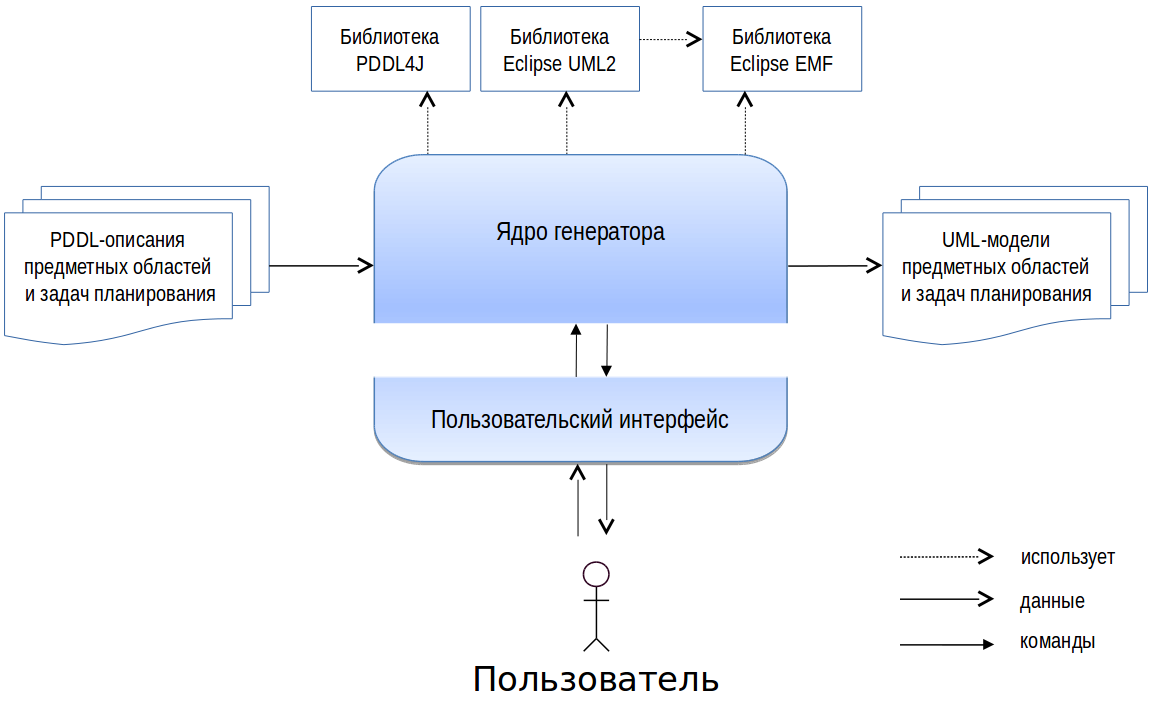
\includegraphics[width=1\linewidth]{system-view}}
    \caption{Общая схема работы средства}
    \label{img:system-view}
\end{figure} 

\begin{figure}[h]
    \center{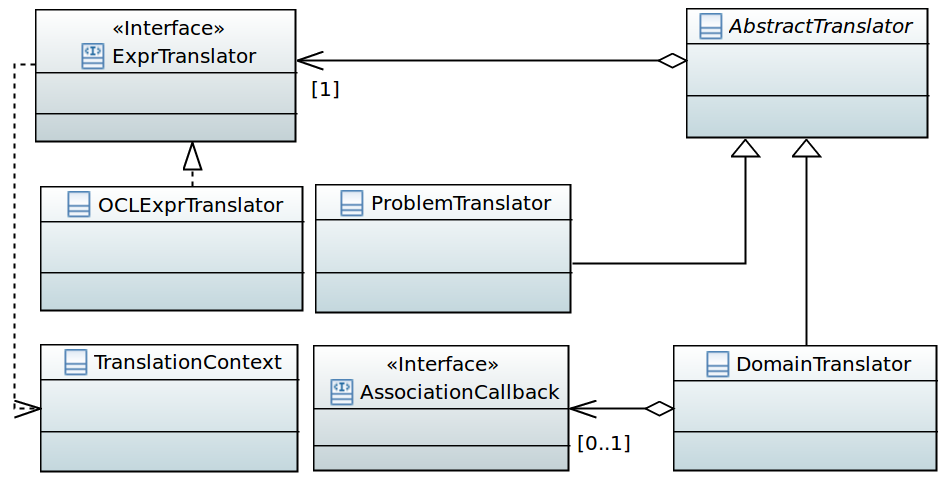
\includegraphics[width=1\linewidth]{artifacts}}
    \caption{Диаграмма для основных компонентов ядра генератора}
    \label{img:artifacts}
\end{figure} 

Общая схема разработанного инструмента показана на рисунке~\ref{img:system-view}. Он состоит из двух частей: первая~-- ядро генератора, которое занимается всеми основными задачами, такими, как управление и обработка ошибок PDDL-парсера, непосредственное создание UML-модели, вторая~-- пользовательский интерфейс (например, консольный), через который происходит взаимодействие с пользователем. Интерфейс использует необходимую функциональность, предоставляемую ядром. Кроме того, интерфейс может зарегистрировать в ядре специальные callback-объекты, которые будут опрашиваться ядром во время уточнения кратностей концов ассоциаций.

В ядре генератора основными являются следующие компоненты:
\\

{
    \renewcommand{\arraystretch}{1.3}
    \small
    \centering
    \begin{tabular}{R{0.45\linewidth}@{\quad-\quad}p{0.45\linewidth}}
        
        \hhline{==}   
            \multicolumn{2}{c}{\parbox{0.9\linewidth}{\rule{0em}{1.5em}\centering{\bfseries <<AssociationCallback>>} -- интерфейс обратной связи с пользователем для уточнения кратности ассоциации}}\\
        \hline    
            Multiplicity checkMultiplicity\newline
            \rule{2em}{0em} (Association assoc, Property end, \newline
            \rule{4em}{0em}Multiplicity supposed) 
            &
            Метод вызывается, когда нужно уточнить утвердить или отклонить кратность \texttt{supposed} у конца \texttt{end} ассоциации \texttt{assoc}. \newline 
            Метод возвращает итоговую кратность данного конца ассоциации\\

        \hhline{==}           
            \multicolumn{2}{c}{ {\bfseries <<Multiplicity>>} -- кратность конца ассоциации}\\ 
        \hline    
            Integer getLow/getHigh ()     &  методы чтения нижней и верхней границы \\
            void setLow/setHigh (Integer) &  методы установки нижней и верхней границы\\

        \hhline{==}
            \multicolumn{2}{c}{\parbox{0.9\linewidth}{\rule{0em}{1.5em}{\centering\bfseries <<AbstractTranslator>>} -- абстрактный базовый класс для трансляторов, инициализирует необходимые для работы с UML статические ресурсы}}\\
        \hhline{==}
            \multicolumn{2}{c}{ {\bfseries <<DomainTranslator>>} -- транслятор предметной области}\\
        \hline   
            void registerCallback(AssociationCallback) & метод регистрирует объект, который будет отвечать на запросы об уточнении кратностей концов ассоциации \\

            Package translate(Domain, List<Problem>) 
            & метод осуществляет трансляцию предметной области, \newline
              список задач планирования нужен только для уточнения кратностей\\
\end{tabular}
\begin{tabular}{R{0.45\linewidth}@{\quad-\quad}p{0.45\linewidth}}
        \hhline{==}
            \multicolumn{2}{c}{ {\bfseries <<ProblemTranslator>>} -- транслятор предметной области}\\
        \hline    
            ProblemTranslator(Package, ExprTranslator)
            & конструктор транслятора, необходимо указать UML-пакет с содержимым предметной области, к которой относится задача и которая уже была транслирована, а также~-- объект, который будет заниматься трансляцией выражений
            \\

            Package translate(Problem) 
            & метод осуществляет трансляцию задачи планирования \\

        \hhline{==}
            \multicolumn{2}{c}{ {\bfseries <<ExprTranslator>>} -- транслятор PDDL-выражений}\\
        \hline
            Constraint translateExpr(TranslationContext ctx, Exp expr) 
            & Метод вызывается, когда нужно транслировать очередное PDDL-выражение \texttt{expr}, трансляция зависит от контекста \texttt{ctx}, в котором находится данное выражение. Метод возвращает новый UML-элемент типа \texttt{Constraint}.\\    

        \hhline{==}
            \multicolumn{2}{c}{ {\bfseries <<TranslationContext>>} -- контекст трансляции}\\
        \hline
            Domain domain &   предметная область задачи планирования \\
            Problem problem & задача планирования \\
            Package domPkg  & UML-пакет, содержащий транслированную предметную область \\
            Package probPkg & UML-пакет, содержащий транслированную задачу планирования \\
            boolean isEffect & флаг, который равен $true$, если выражение находится в эффекте \\
            \multicolumn{2}{c}{\rule{0em}{1.5em} \parbox{0.9\linewidth}{$*$ перечисленные поля контекста являются публичными, в каждом конкретном случае могут быть инициализированы не все из них}}\\

        \hhline{==}
            \multicolumn{2}{c}{ {\bfseries <<OCLExprTranslator>>} -- транслятор PDDL-выражений на язык OCL}\\
        \hline
            Constraint translateExpr(TranslationContext ctx, Exp expr) 
            & реализация метода интерфейса, осуществляющая трансляцию таким образом, что в результирующее ограничение \texttt{Constraint} будет помещен элемент \texttt{ValueSpecification} типа \texttt{LiteralString}, в который будет записана соответствующая OCL строка \\
    \end{tabular}
}
\\[5pt]

Отношения между сущностями, перечисленными в таблице, показаны на рис.~\ref{img:artifacts}.
Кроме ядра генератора был реализован консольный пользовательский интерфейс, архитектура которого предельно проста и не нуждается в детальном рассмотрении. Единственное, что стоит упомянуть~--- для консольного интерфейса создается объект, реализующий интерфейс \texttt{AssociationCallback}, который затем регистрируется в ядре. Когда вызывается нужный метод этого объекта, для уточнения кратности конца ассоциации организуется необходимый консольный диалог с пользователем.

\section{Пример работы генератора}

Рассмотрим работу средства на примере предметной области ``Обедающие философы'', которая уже неоднократно упоминалась ранее. Инструмент вызывается командой \texttt{pddl2uml}, у которой один обязательный аргумент~--- путь к файлу с описанием предметной области, необязательные аргументы~--- это пути к файлам м задачами. Кроме этого, программа может воспринимать набор дополнительных опций, указывающих, например, нужно ли выдвигать предположения о кратностях (\texttt{-m}), нужно ли просить пользователя утвердить эти предположения в интерактивном режиме (\texttt{-i}), нужно ли спросить пользователя о кратности даже если предположений выдвинуть не удалось (\texttt{-a}) и т.д.

\begin{alltt}\small
    pddl2uml philosophers.pddl p3.pddl -m -i
\end{alltt}

В ходе выполнения этой команды программа будет генерировать две модели: для предметной области и для задачи. Во время генерации ассоциаций программа проанализирует задачу и предложит пользователю утвердить ограничения на кратность конца ассоциации \texttt{left}:

\begin{alltt}\small
    Found that association end "Philosopher.left" can be constrained as [0..1].
    Accept? [y/Y/n/N/N!/p/c]:
\end{alltt}

Значение ответов на этот вопрос следующее: \texttt{y}~-- утвердить предложенный вариант, \texttt{Y}~-- утвердить предложенный вариант и все следующие, \texttt{n}~-- отклонить вариант и предложить другой, если есть возможность, \texttt{N}~-- отклонить все варианты для данного конца ассоциации (т.е. оставить её максимально неопределенной \texttt{[*]}), \texttt{N!}~-- отклонить предложенный вариант и все следующие, \texttt{p}~-- если ранее было предложен вариант для текущего конца, отклоненный нажатием \texttt{n}, то предложить его заново, \texttt{c}~-- ввести значение кратности вручную (custom).

Предположим, что мы отказались, дав ответ \texttt{n}, тогда будет предложен новый вариант:

\begin{alltt}\small
    [Continued] 
    Found that association end "Philosopher.left" can be constrained as [1].
    Accept? [y/Y/n/N/N!/p/c]:
\end{alltt}

Теперь предположим, что мы захотели ввести свое значение \texttt{[0..1]} (пусть даже уже предложенное ранее), тогда мы отвечаем \texttt{c} и вводим новое значение кратности:

\begin{alltt}\small
    New constraint: 0..1
\end{alltt}

Результат ограничения кратности конца ассоциации уже рассматривался ранее: получаемые OCL выражения станут гораздо проще.

В конечном счете программа создает две модели \texttt{philosophers.uml} и \texttt{p3.uml} в формате XMI. Полученные модели можно открыть, например, при помощи Eclipse Papyrus.
\\

Для тестирования реализованных возможностей использовались несколько предметных областей и задач к ним:

ПО ``Логистика''~--- предметная область, в которой описываются различные грузоперевозки наземным и воздушным способом. Она выбиралась потому, что в ней присутствует большое количество связей тип-подтип и ассоциаций.

ПО ``Обедающие философы''~--- несложная предметная область, в которой неявно присутствуют ограничения на кратности концов ассоциаций, поэтому её можно использовать для тестирования методов восстановления информации.

ПО ``Мир кубиков''~--- предметная область,  в которой присутствует рефлексивная ассоциация. Помимо этого она может быть описана с использованием объектных флюент, что даст возможность тестировать преобразование флюент.

Примеры предметных областей можно найти в приложении к работе. 
%\subsection{``Портфели''}


%\subsection{``Ханойские башни''}


%\subsection{``Логистика''}


\newpage